% Template for ICIP-2012 paper; to be used with:
%          spconf.sty  - ICASSP/ICIP LaTeX style file, and
%          IEEEbib.bst - IEEE bibliography style file.
% --------------------------------------------------------------------------

\documentclass{article}
\usepackage{spconf,amsmath,graphicx}
\usepackage{amssymb}
\usepackage{bibentry}
\nobibliography*
% Example definitions.
% --------------------
\def\x{{\mathbf x}}
\def\L{{\cal L}}

% Title.
% ------
\title{Recognizing Chess Pieces Using an Object Ensemble Approach}
%
% Single address.
% ---------------
\name{Geoffrey Kao, Ruiyang Hu\thanks{We are indebted to Professor Antonella and Solomon Garber for their expertise and time.}}
\address{Brandeis University}
%
% For example:
% ------------
%\address{School\\
%	Department\\ 
%	Address}
%
% Two addresses (uncomment and modify for two-address case).
% ----------------------------------------------------------
%\twoauthors
%  {A. Author-one, B. Author-two\sthanks{Thanks to XYZ agency for funding.}}
%	{School A-B\\
%	Department A-B\\
%	Address A-B}
%  {C. Author-three, D. Author-four\sthanks{The fourth author performed the work
%	while at ...}}
%	{School C-D\\
%	Department C-D\\
%	Address C-D}
%
\begin{document}
%\ninept
%
\maketitle
%
\begin{abstract}
\hspace{\parindent} This paper discusses methods on taking in a visual image of a physical chessboard with pieces and returning a digitially reconstructed computer representation of the board. Although chess piece classification has been a topic previously explored in the past, previous works have primraily focused on using local feature descriptors for object classification. In this paper, we instead adopt a deep learning approach, relying on generic descriptors extracted from a convolution neural network for feature description. Our empirical results supports the recent literature of the superiority of generic feature descriptors extracted from convolutional neural networks. In comparison to local feature descriptors, such as SIFT, image classifiers based off of global features greatly outperform their local features counterparts. We further explore an ensemble approach consisting of both local feature descriptors and global feature descriptors, an attempt that proves less promising than a purely generic feature descriptors approach.\end{abstract}
%

%
\section{Introduction}
\label{sec:intro}

\hspace{\parindent}For chess players, tracking the movement of chess pieces is a task that proves tedious, resulting in both wasted time and inaccurate recordings during fast games. Recent work in the field has emerged on digitally reconstructing chess boards based off of input images, yet the current state of classifying chess pieces has not advanced enough for consistently accurate digital reconstructions. The benefits of being able to accurately digitize chessboards would be immense, allowing chessplayers to focus on playing,\cite{densenet} while allowing spectators to instantly compare real-time games with other historical examples. Furthermore, the benefits of accurate chess piece detection can be extrapolated to other applications of object classification such as facial recognition. \newline
\indent Our approach to classifying pieces iterates upon previous works, many of which have focused on using local feature descriptors such as SIFT and HOG to extract features from training data  . These features are chosen for images properties that should lend itself to robustness such as  scale invariance or rotation invariance, yet in practice, creating a robust image classifier has proved quite difficult. Recent advances in the deep learning field have suggested better results may be found in transitioning away from these local feature descriptors, and instead adopting an approach that depends more heavily on generic global feature descriptors such as feature maps. However,more progress has not been made because of the absence of a robust, labelled dataset of chess boards and pieces. The lack of a large dataset has been assumed to result in poor performance on trained convolutional neural networks by making them prone to overfitting. However, as we will show in our results, this assumption is overblown. Despite a relative small training set to work with, we still achieve  high performance through our use of a feature map extracted from a convolutional neural network. The results significantly outperform any results from approaches that solely utilize local feature descriptors. We conclude the paper by discussing our results from an ensemble approach that incorporates both local and deep features. 

\section{Background}
\label{sec:intro}
\hspace{\parindent}Chess is a player versus player board game that consists of a 8x8 board of alternating white and black squares. Each player has 16 pieces of the same color- usually either white or black. A player has 8 pawns, 2 rocks, 2 knights, 2 bishops, and a queen, and a king. Squares are denoted an algebraic notation with a column  assigned a letter and each row assigned a number. Thus, at the start of the game, the white player should have the square a1 to his/her immediate left and square h1 to his/her immediate right. On the other side of the board, the black player should have square h8 to his/her immediate left and square a1 to his/her immediate right. Our end goal is to take in a visual image of a board and return a digital reconstruction of a board with square assignment for each piece. Thus, we would like to ideally be able to return to a user that a white pawn is found on b5 or a black queen is placed on h4. To achieve this, board deconstruction and piece identification must be successfully achieved. For this paper, piece identification will be the primary topic of discussion, although a brief discussion of board deconstruction can be found in the endnotes.%
\section{Methodology}
\label{sec:format}
\hspace{\parindent}The overall architecture consists of a combination of deep and local feature descriptors. We extract descriptors from the second-to-last fully connected layer of a fully connected convolution network along with a vector representation of a SURF feature descriptor trained on on our training set. We aggregate the features and then train a linear support vector machine (SVM) to classify chess piece type. Our database consists of a combination of pictures taken manually along with pictures that were extracted using a cutting software we've implemented. Per piece type, we have at least 50 images, all of which are taken from the same chessboard and chess piece set. We also have built a smaller extraneous test set that consists of randomly chosen images from the internet. Unfortunately, due to the limited availability of images that meet our criteria, our internet test set is not robust enough for comprehensive testing. Figure 1 displays a sample image from our database.
\newline
\begin{figure}[htb]

\begin{minipage}[b]{1.0\linewidth}
  \centering
  \centerline{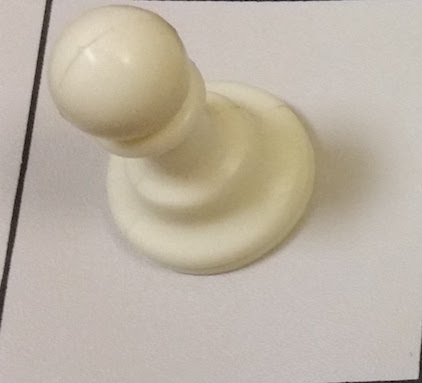
\includegraphics[width=7.5cm]{sample}}
%  \vspace{2.0cm}

\end{minipage}
%

%
\caption{Sample pawn}
\label{fig:res}
%
\end{figure}
\subsection{Local Descriptors}
\label{ssec:subhead}

\hspace{\parindent}Local features were extracted over the images in the database using the Speeded up Robust Features descriptor (SURF) [3]. SURF is a feature descriptor is similiar to the Scale-invariant feature transform descriptor (SIFT)[4], both of which are scale and rotation invariance and operate by finding keypoints. Because SIFT uses a difference of gaussian approach to extract keypoints, SIFT can be quite costly to run. Thus, in the interest of reducing our already lengthy local feature extraction run time, we employ SURF as our feature descriptor instead of SIFT. More work can be done to see if this choice has an impact on our results.\newline
\indent The main bottleneck in extracting the local features stem from our local feature encoding strategy. We utilize a standard "bag of visual words" approach that has been employed by others for similar image classification problems [5], extracting SURF vectors for each image in our training set. Through k-means clustering over all vectors, we produce a "codebook" of "codewords" that represent the center of these clusters. Keypoints are thus mapped to keywords and classes can be represented by the histogram of codwords.\newline
\indent Clustering is a time consuming process. Due to limited access to extensive computational resources, we were forced to run the clustering on a local laptop. For a laptop with a Intel core i7 processor and a Nvida GeForce GTX 1080 graphics card, the SURF feature extraction and encoding over our limited training set took an average of 45 minutes. For real-time extraction, this method is simply not feasible, and others hoping to replicate our research under more limited time constraints should seek to utilize other encoding strategies.
\subsection{Global Feature Descriptors}
\label{ssec:subhead}
\hspace{\parindent} In order to extract generic global feature descriptors, we utilize Resnet-50, a pretrained neural network, released by Microsoft, consisting of 50 layers[6]. As the name suggests, Resnet-50 adotps a residual learning approach that differs from traditional deep learning networks. Instead of calculating features, the network calculates residuals, the subtraction of features learned from one layer to another. The benefits of the residual learning approach is that we can train deeper neural networks without additional error. For our purposes, we believed that a 50 layer network was sufficient. Additional layers provided by a network such as Resnet-101 or Resnet-250 could potentially result in better feature extraction; however, we found that the fast inference timefrom Resnet50 resulted in sufficiently adequate results.\newline
\indent
One of the limitations of using Resnet is that it requires RBG images that are 224-by-224 in size. We thus had to preprocess our training set by transforming all our images into the necessary size before feeding them into the neural network. Selecting which deep layer to extract is a question we faced, but we ultimately ended up choosing to extract the layer right before the classificaiton layer. Although some have used the classification layer for similiar purposes, we believed the classification layer to be too image specific, and not robust enough to noise. Figure 2 displays a visual representation of the first layer of our network.
\newline
\begin{figure}[htb]

\begin{minipage}[b]{1.0\linewidth}
  \centering
  \centerline{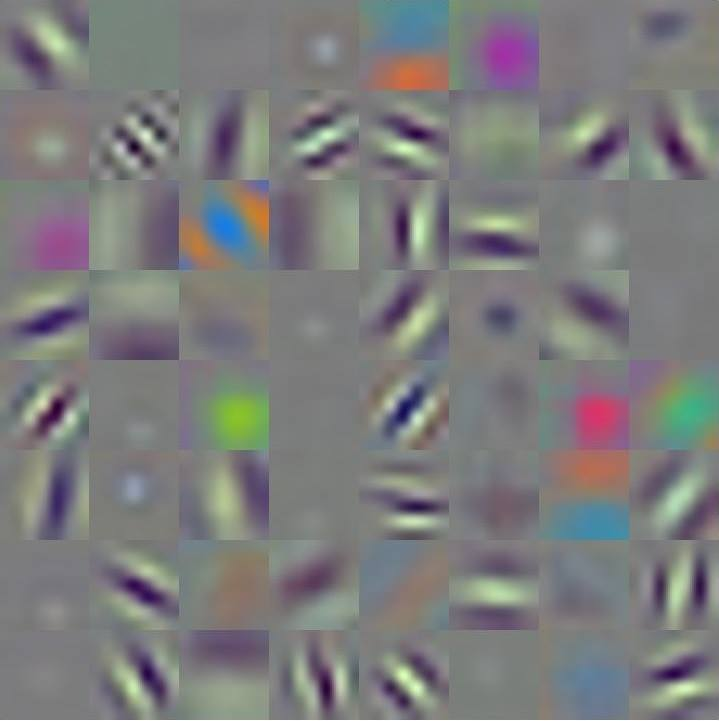
\includegraphics[width=8.5cm]{firstLayer}}
%  \vspace{2.0cm}

\end{minipage}
%

%
\caption{First convolutional layer weights}
\label{fig:res}
%
\end{figure}
\subsection{Combining  Descriptors}
\label{ssec:subhead}
\hspace{\parindent}For image classification, other architectures have been proposed to incorporate both local and deep features [7]. Typically, these architectures consist of separate classifiers trained separately on the local and deep features, before outputting a final prediction label decided through a predefined voting mechanism. In designing our architecture, we modified this traditional approach by instead relying on only one classifier- a linear support vector machine. Although other classifiers were explored such as a logistic regression classifier and a Gaussian SVM, our empricial results were most optimal using a linear support vector machine. We credit our robust feature descriptors for allowing us to obtain high performance results despite a relatively simple classifier approach.\newline
\indent Combining the feature map from Resnet-50 and the feature vector corresponding to the SURF features proved quite difficult. Simple concatentation cannot be done due to the distinct dimensonalities. As a solution, we've chosen a suboptimal solution of flattening the feature map down to a feature vector and then aggregating the flattened vector with the SURF feature vector. 
\newline

\begin{figure}[htb]

\begin{minipage}[b]{1.0\linewidth}
  \centering
  \centerline{(a) Results for SURF Linear SVM, mean: .5443}\medskip
  \centerline{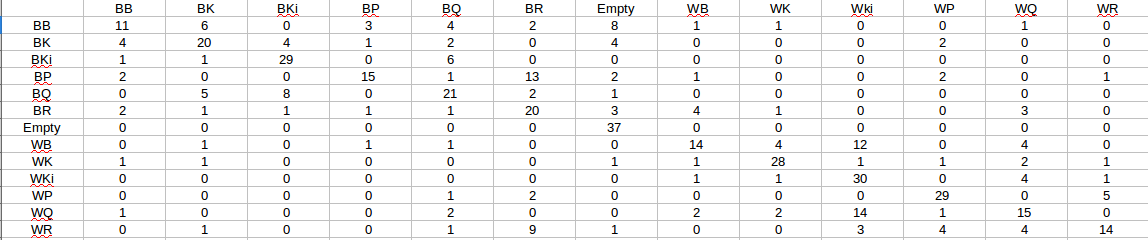
\includegraphics[width = 9.0cm, height = 3 cm]{firstResults}}
  \vspace{1.0cm}
\end{minipage}
%%\vspace{2.0cm}
\begin{minipage}[b]{1.0\linewidth}
 \centering
  \centerline{(b) Results for CNN Linear SVM, mean: .9605}\medskip
  \centerline{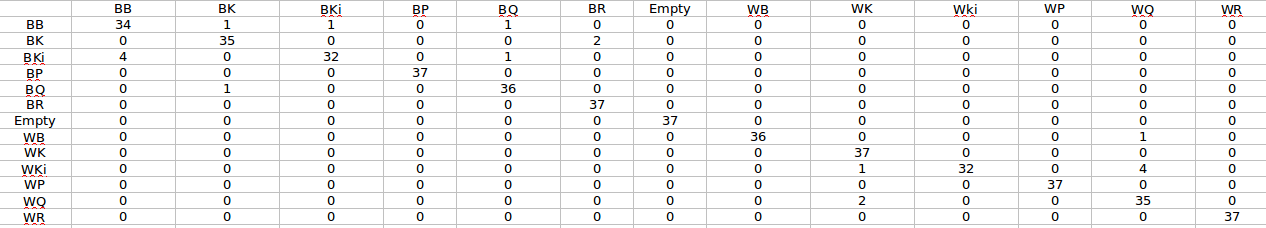
\includegraphics[width = 9.0cm, height = 3 cm]{secondResults}}
  \vspace{1.0cm}
\end{minipage}
\hfill
\begin{minipage}[b]{1.0\linewidth}
 \centering
  \centerline{(c) Results for SURF and CNN Linear SVM, mean: .9543}\medskip
  \centerline{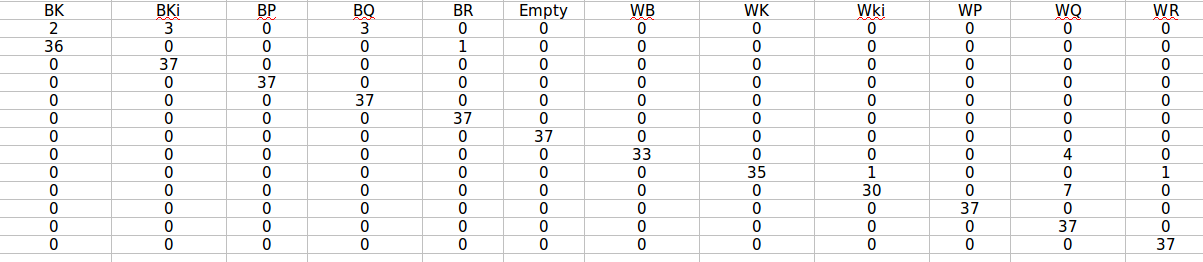
\includegraphics[width = 9.0cm, height = 3 cm]{thirdResults}}
  \vspace{1.0cm}
\end{minipage}
%
\caption{Confusion Matrixes Over Different Feature Sets}
\label{fig:res}
%
\end{figure}
\section{Results}
\label{sec:pagestyle}

\hspace{\parindent}The results of running the linear SVM classifier can be found in figure 3 with each table representing a confusion matrix for the different feature descriptors. The labels on the left represent the actual labels, while the labels on the right represent the predicted labels. The first letter of each label represents the color, thus, BB stands for black bishop while WK stands for white king.\newline
\indent Table A represents the confusion matrix for the linear SVM classifier trained on only the SURF feature descriptor. As expected, image classification performed on using only the SURF feature descriptors performs quite poorly. The classifier in this scenario has trouble distinguishing similar looking pieces such as kings and queens. For especially distinct test cases such as an empty square, the classifier is highly acurrate. \newline
\indent Table B represents the confusion matrix for the linear SVM classifier trained on the feature map extracted from Resnet-50. The results speak for themselves. With a 96 percent accuracy rate, the global feature descriptor classifier achieves high accuracy in identifying pieces. Our results further supports the growing literature on the superiority of deep learning approaches for object recognition tasks. The classifier however occasionally still occasionally struggles with distinguishing between similiar looking pieces. Similar to the linear SVM classifier trained on only the SURF feature descriptor, the CNN SVM classifier will occasionally erroneously identify white kings as white queens and vice versa. This failure could potentially be atrributed to overfitting from our relatively small training set.
\newline\indent Table C represents the confusion matrix for the linear SVM classifier trained with both the SURF feature vector and the feature map extracted from Resnet-50. The results are a bit disappointing with a minor drop in accuracy compared to the a classifier trained on solely the feature map. This result however is not completely surprising. In a feature map, the weights are location sensitive, and correspond to geographical locations within an image. Flattening the feature map down to a one-dimensional feature vector results in important information about the locational relationship between the feature map and the output image being lost.
\section{Possible Improvements}
\label{sec:typestyle}
\hspace{\parindent} Because of the many design choices we faced in implementing our classifiers and neural network, there are many avenues for future exploration. The biggest struggle we faced, aside from encoding for the the SURF feature descriptor, was how to adequately merge the feature map and the SURF feature descriptor to train our sole classifier on. Our approach is suboptimal because we incur a significant loss of information by flattening the feature map. Ideally, we want to complement the convolutional neural networks ability to extract descriptive features with rotation and scale invariance benefits of SIFT or SURF without sacrificing breadth. Possible techniques to explore include principal component analysis (PCA) and Baynesian networks. \newline
\indent Our local features encoding strategy also leaves a lot to be desired. Because of the k means clustering, extraction time is quite lengthy. As the database of images grow, the inference time will only grow exponentially. Other types of encoding strategies employed by others have included Fisher vectors and Vector of Linearly Aggreated Descriptors (VLAD). Universally, encoding time still remains a major bottleneck for object classification using local feature descriptors.
\newline\indent In designing residual learning network, we made some underlying assumptions that need further analysis. For one, we assume that our use of Resnet-50 is sufficiently powerful and that the benefits of utilizing a deeper network such as Resnet-101 is marginal. Furthermore, we base our feature map on the second-to-last layer of our convolutional neural network. More done needs to be to see whether additional accuracy can be obtained through optimizing layer choice.


\section{Conclusion}
\label{sec:typestyle}
\hspace{\parindent} 
Code for our project can be found on github.com/gkao123. In this paper, we explore an object ensemble approach utilizing both local and deep feature descriptors to classify pieces, and compare it to similar classifiers that utilize only either local or deep features. Although the results are a bit disappointing, more work must be done before conclusively deciding the viability of an object ensemble approach. Our work however further corroborates the power of deep learning for object classification tasks even on limited training sets. 

\section{Endnotes}
\label{sec:copyright}
\hspace{\parindent}As mentioned earlier in the paper, we've designed a board deconstruction software by utilizing a preexisting library in Matlab. Matlab has a prebuilt library called detectCheckberboard() [8] that uses a corner detection approach through Harris points to detect squares on a checkerboard. Through pixel location, we use matlab's image extraction tools to extract 64 images from one input image, with each image corresponding to a square. We've optimized it further to incorporate rotation features to standardize the pictures taken. Although we've made some progress, the software still struggles with extracting empty squares. 


\bibliographystyle{alpha}
\bibliography{bibl.bib}

\end{document}
